\documentclass[11pt, fleqn]{article}

\usepackage[letterpaper, margin=0.7in]{geometry}
\usepackage{graphicx}
\usepackage{subcaption}
\usepackage{cleveref}
\usepackage{listings}
\usepackage{multicol}
\usepackage{tikz}
\usepackage{bm}
\usepackage{minted}
\usetikzlibrary{arrows}
\usepackage{wrapfig}
\usepackage{amsmath}
\usepackage{amssymb}
\usepackage[section]{placeins}
\usepackage{pgfplots,wrapfig}  
\pgfplotsset{compat=newest} 
\pgfplotsset{plot coordinates/math parser=false} 
\newlength\figureheight 
\newlength\figurewidth 
\setlength{\parindent}{0pt}
\newcommand\tab[1][1cm]{\hspace*{#1}}
\usepackage{algorithm}
\usepackage[noend]{algpseudocode}

\let\oldReturn\Return
\renewcommand{\Return}{\State\oldReturn}

\raggedbottom

\begin{document}

\begin{center}

\Large{COMP6212 Assignment 4 : Shakib-Bin Hamid 25250094 sh3g12}

\end{center}

\section{Kalman Filter}

Lets suppose there a data generative process is a linear of its past values, i.e. the current process process parameters are a linear combination of previous process parameters. In this respect we can calculate the process parameters by minimising the least squared error between the prediction and the true values, $\bm{\omega} = (\bm{Y}^t\bm{Y})^{-1}\bm{Y}^t\bm{f}$, where $\bm{Y}$ is the input data and $\bm{f}$ is the target. But this method requires calculating a new $\bm{Y}^{-1}$ (a $O(n^3)$ operation) when we receive any new data. If the process is generating a time series data (getting data one at a time), then online updating the parameters can be incredibly costly.\\

However, it can be shown that we can calcuate new parameters without calculating a new inverse, $\bm{\omega}_n = \bm{\omega}_{n-1} + L \times (f_n - \bm{\omega}_{n-1}^ty_n)$. It means that we can calculate new parameters by updating the old parameters with the scaled prediction error on new data using the old parameters. Of course we need to assume some initial values for our parameters. But, we still do not account for any noise in our process.\\

In a Kalman Filter, we may assume a process $\bm{\omega}_n = \bm{A}\bm{\omega}_{n-1} + \bm{\epsilon}(n)$, where the process noise $\bm{\epsilon} \sim \mathcal{N}(0, \bm{Q})$. Here we can assume that our parameters are a linear transformation of previous parameters corrupted by Gaussian noise. Similarly, we can assume that our observation $f_n = \bm{\omega}_n\bm{y}_n + \xi(n)$, where observation noise $\xi \sim \mathcal{N}(0, R)$.\\

\cite{mahler} claims that we can predict the monthly S\&P 500 index using a Kalman filter. In order to verify his claim, I have built Algorithm \ref{alg:kalman} -

\begin{algorithm}[H]
\caption{S\&P 500 Index Prediction using a Kalman Filter}
\label{alg:kalman}
\begin{algorithmic}

\Procedure{Kalman}{$\bm{s}, o, \alpha, R$} 

\State \Comment{$\bm{s}$ = index, $o$ = order, $\alpha$ = is a constant, R = observation noise variance}

\State $N$ = $size(\bm{s}, 1)$; \Comment{Number of months}
\State $\bm{Y}$ = $zeros(N - o + 1, o)$; \Comment{Input data in $o$ order windows}
\State $\bm{W}$ = $zeros(N - o + 1, o)$; \Comment{Weights at every point}
\State $\bm{e}$ = $zeros(N - o + 1, 1)$; \Comment{Prediction error at every point}
\State $\bm{K}$ = $zeros(N - o + 1, o)$; \Comment{Kalman gain at every point}

\State

\State $\bm{A}$ = $\bm{I}_o$ \Comment{$\bm{I}_o$ is the $o$ order Identity}
\State $\bm{Q}$ = $\alpha\bm{I}_o$ \Comment{Process noise covariance}

\State

\State $\bm{P}$ = $ones(o)$ \Comment{Inital value of $\bm{P}$}
\State $\bm{W}(1,:)$ = $o^{-1}ones(1,o)$

\State

\For {$i \gets 1,N-o$}

	\State $\bm{Y}(n, :)$ = $\bm{s}(i:i+o-1)$ \Comment{Input is last $o$ months' index}

	\State

	\State $\hat{\bm{w}}$ = $\bm{A}\bm{W}(n-1, :)^t$ \Comment{Prediction}
	\State $\hat{\bm{P}}$ = $\bm{A}\bm{P}\bm{A}^t$ + $\bm{Q}$ 

	\State
	
	\State $\bm{e}(n)$ = $\bm{s}(n+o-1)$ - $\bm{Y}(n, :)\hat{\bm{w}}$ \Comment{Prediction Error}
	\State $\bm{K}(n,:)$ = $(\hat{\bm{P}}\bm{Y}(n, :)^t)/(R + \bm{Y}(n, :)\hat{\bm{P}}\bm{Y}(n, :)^t)$ \Comment{Kalman Gain}

	\State

	\State $\bm{W}(n, :)$ = $\bm{W}(n-1, :) + \bm{K}(n,:)\bm{e}(n)$ \Comment{Correction}
	\State $\bm{P}$ = $(\bm{I}_o - \bm{K}(n,:)^t\bm{Y}(n, :))\bm{P}$ 

\EndFor

\EndProcedure
\end{algorithmic}
\end{algorithm}

Here the input at each point in time is past $o \in {2, ..., N-1}$ index values. Observation noise $R$ is taken as the residual variance from an autoregression model using \texttt{ar} function of Matlab's System Identification Toolbox. Process noise covariance needed to be tuned via $\alpha$. From Figure \ref{fig:error-vs-alpha-order-3} (where I have plotted the cumulative sum of prediction error as a function of $\alpha$ for a 3rd order filter), we can say that $10^{-3}$ is a reasonable value for $\alpha$.\\

\begin{figure}[!h]
  	\centering
  	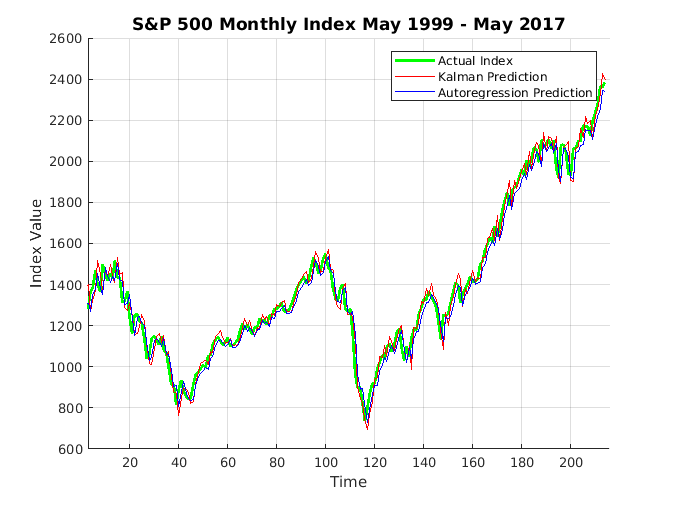
\includegraphics[width=0.5\textwidth]{kalman-autoreg-pred.png}
	\caption{Kalman \& Autoregression Prediction}
	\label{fig:kalman-autoreg-pred}
\end{figure}

\begin{figure}[!h]
    \centering
    \begin{subfigure}[b]{0.45\textwidth}
        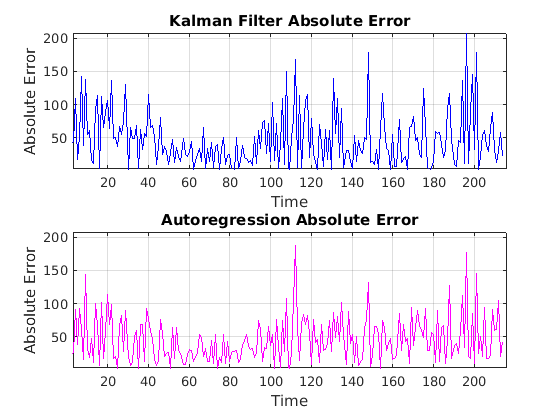
\includegraphics[width=\textwidth]{kalman-autoreg-error.png}
		\caption{Index Prediction Absolute Error}
		\label{fig:kalman-autoreg-error}
    \end{subfigure}
    ~ 
    \begin{subfigure}[b]{0.42\textwidth}
        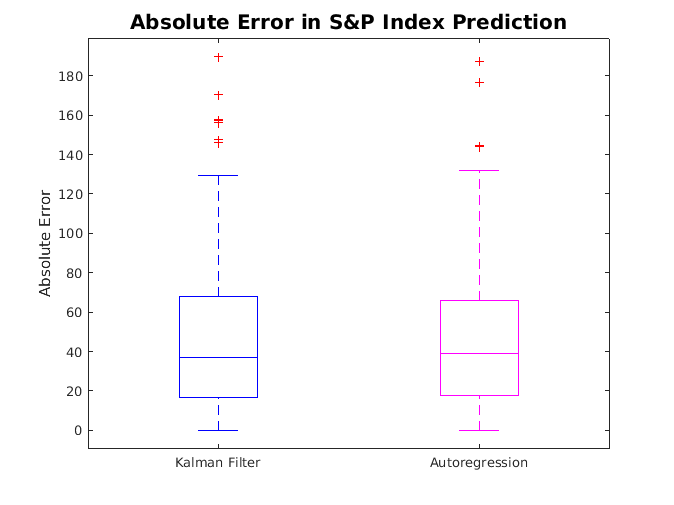
\includegraphics[width=\textwidth]{kalman-autoreg-error-boxplot.png}
		\caption{Index Prediction Error Comparison}
		\label{fig:kalman-autoreg-error-boxplot}
    \end{subfigure}
    \caption{Prediction Error}
	\label{fig:prediction-error}
\end{figure}

\begin{figure}[!h]
    \centering
    \begin{subfigure}[b]{0.45\textwidth}
        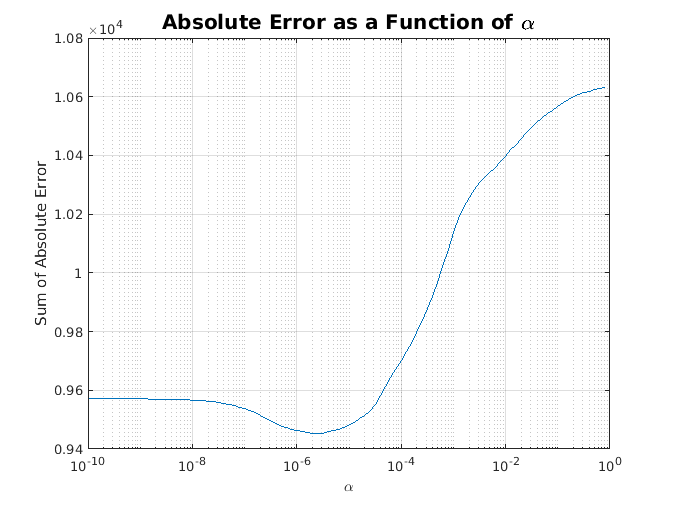
\includegraphics[width=\textwidth]{error-vs-alpha-order-3.png}
	\caption{Cumulative Absolute Error as a Function of $\alpha$}
	\label{fig:error-vs-alpha-order-3}
    \end{subfigure}
    ~ 
    \begin{subfigure}[b]{0.42\textwidth}
        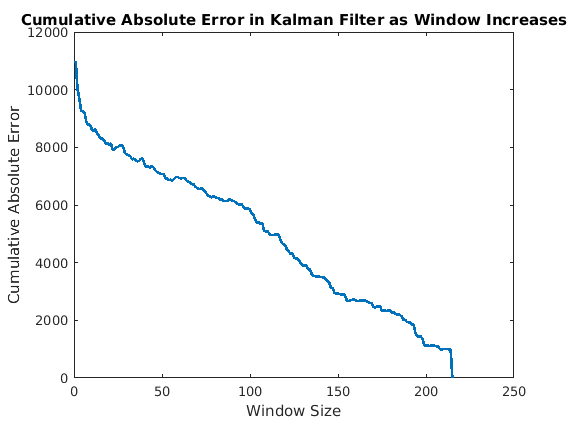
\includegraphics[width=\textwidth]{kalman-error-vs-window.png}
		\caption{Index Prediction Error Comparison}
		\label{fig:kalman-error-vs-window}
    \end{subfigure}
    \caption{Cumulative Absolute Error as a function of $o$ and $\alpha$}
	\label{fig:o-alpha-error}
\end{figure}

\begin{figure}[!h]
  	\centering
  	
\end{figure}

\begin{thebibliography}{9}
\bibitem{mahler} 
N. Mahler, "Modeling the S \& P 500 index using the Kalman filter and the LagLasso," in \textit{Machine Learning for Signal Processing, 2009. MLSP 2009. IEEE International Workshop on, Sept 2009}, pp. 1–6.

\end{thebibliography}

\end{document}












































